\documentclass[12pt]{article}

\usepackage[spanish]{babel}
\usepackage[utf8x]{inputenc}
\usepackage{amsmath}
\usepackage{amsthm}
\usepackage{graphicx}
\usepackage{amsfonts}
\usepackage{color}
\usepackage{enumerate}
\newtheorem*{myteo}{Teorema}
\newtheorem*{mydef}{Definición}

\title{Kernel Trick}
\author{Paola Arce \and Raquel Pezoa}

\begin{document}
\maketitle

\section{Idea Intuitiva de Kernels}
Supondremos que tenemos un conjunto con dos clases de objetos. Al llegar un nuevo objeto, interesa saber a qué clase pertenece, por lo tanto, se está frente a \textbf{el problema} de clasificación de objetos \cite{smola}.

Para poder realizar aquella clasificación en el contexto de máquinas de aprendizaje es necesario contar con \textbf{datos de entrenamiento}: $$\{ (x_k,y_k)\}_{k=1,\cdots,n} \in X \times \{-1,1\},$$ 

\noindent donde $X$ es simplemente --por el momento-- un conjunto no vacío y $x \in X$ corresponde al dato de entrada (también denominados casos, observaciones, patrones, etc.) e $y$ corresponde a la salida o etiqueta asociada al dato de entrada.

Cuando aparece un nuevo dato de entrada $x \in X$, se desea predecir su etiqueta $y \in \{-1,1\}$, es decir, se debe escoger un valor de $y$ que de alguna manera sea \textbf{similar} a los datos de entrenamiento $(x,y)$. Esta predicción con base en los datos de entrenamiento, se denomina \textbf{generalización}, es decir, se trata de una predicción de la etiqueta de los nuevos datos de entrada basándonos en su similitud con los datos de entrenamiento.

Para medir la similitud entre datos, se pueden usar diversas funciones. En el caso de las etiquetas $y \in \{-1,1\}$, caracterizar la similitud es simple, ya que sólo pueden ocurrir dos situaciones: o bien las etiquetas son idénticas o bien son diferentes. En el caso de los datos de entrada, la caracterización de su similitud es un poco más compleja, y es un aspecto central en el campo de las llamadas máquinas de aprendizaje.

Consideremos una medida de similitud de la forma:

\begin{equation}
\begin{tabular}{ll} \\
$k:$ & $X \times X \rightarrow \mathbb{R}$ \\ 
   & $(x,x') \rightarrow k(x,x')$ \\
\end{tabular}
\end{equation}

\noindent donde $k$ es una función que recibe dos parámetros, $x$ y $x'$, y cuya salida es un valor real que caracteriza la similitud de ambos parámetros. Supondremos que $k$ es una función simétrica, es decir, $k(x,x')= k(x',x) \quad \forall x, x' \in X$. Esta función $k$, es denominada \textbf{kernel}.

%La forma general de los kernels, son un tanto complejas de estudiar, así que se comenzará con un caso particular para llegar a entender su forma general. 

Un ejemplo de medida de similitud simple es una basada en el \textbf{producto interno}\footnote{Revisar en Sec. \ref{sec:def} la definición de producto interno a partir de formas hermitianas.} (también conocido como producto interno o producto escalar). Por ejemplo, para los vectores $x, x' \in \mathbb{R}^n$, se define el \textbf{producto punto canónico} de la siguiente manera:

\begin{equation}
\langle {\bf x}, {\bf x' } \rangle := \sum \limits_{i=1}^{N} [{\bf x}]_i [{\bf x' }]_i 
\end{equation}

\noindent donde $[x]_i$, resp.  $[x']_i$, denota la $i$-\'esima
componente del vector $x\in\mathbb{R}^N$, resp.  $x'\in\mathbb{R}^N$.









\section{Espacios de Hilbert}

\begin{mydef}
Un producto interno $\langle\cdot,\cdot\rangle$ sobre un espacio vectorial
{\bf real} $X$ es una aplicaci\'on 
$\langle\cdot,\cdot\rangle:X\times X\to\mathbb{R}$,
que es lineal con respecto al primer y al segundo argumento
y es tal que 
$\langle\mathbf{x}, \mathbf{x}\rangle\geq0$ para todo $\mathbf{x}\in X$
y $\langle\mathbf{x}, \mathbf{x}\rangle=0$ si y s\'olo si $\mathbf{x}=0$.
\end{mydef}

\begin{mydef}
Un espacio de Hilbert $H$ sobre $\mathbb{R}$ es un espacio vectorial real
equipado con un producto interno $\langle\cdot,\cdot\rangle$, tal que
es completo con respecto a la norma
$\|\mathbf{x}\|^{2}= \langle\mathbf{x},\mathbf{x}\rangle$,
$\mathbf{x}\in H$.
\end{mydef}

Si bien todo espacio de Hilbert es un espacio de Banach, 
no todo espacio de Banach es un espacio de Hilbert.

\begin{mydef}
Un espacio de Banach $(X,\|\cdot\|)$ es un espacio de Hilbert
si y s\'olo si la norma $\|\cdot\|$ del espacio satisface la
identidad del paralel\'ogramo:
$$
\|\mathbf{x}+\mathbf{y}\|^2+\|\mathbf{x}-\mathbf{y}\|^2
= 2\|\mathbf{x}\|^2+2\|\mathbf{y}\|^2\quad
\text{para todo}\quad \mathbf{x},\mathbf{y}\in X\,.
$$
\end{mydef}

\begin{mydef}
Un espacio pre-Hilbert es un espacio vectorial equipado con un producto
interno o escalar.
Por eso, los espacios pre-Hilbert se denominan tambi\'en espacios con
producto interno.
No se exige que los espacios pre-Hilbert sean {\bf completos}.
Si adem\'as son completos, entonces se trata de espacios de Hilbert.
\end{mydef}

%Un espacio de Hilbert $H$ es un espacio vectorial equipado con un producto interno o producto escalar $\langle \cdot,\cdot \rangle$:

%\begin{equation}
%(H,\langle \cdot,\cdot \rangle) \Longrightarrow \text{ completo c/r  %}||\mathbf{x}||^2= \langle \mathbf{x},\mathbf{x} \rangle
%\end{equation}


%\begin{myteo}[de representación de Riesz]
%Si $H$ es un espacio de Hilbert y $\varphi$ un funcional %lineal y continuo:
%\begin{equation}
%\varphi: H \rightarrow \mathbb{C} \Longrightarrow \exists! %y_{\varphi} \in H \qquad \forall x \in H: \qquad \varphi(x) %= \langle x,y_{\varphi}\rangle 
%\end{equation}
%$y_{\varphi}$ se le denomina el representante.
%\end{myteo}


\begin{myteo}[de representación de Riesz]
Si $H$ es un espacio de Hilbert sobre un cuerpo escalar $\mathbb{K}$
($\mathbb{K}$ puede ser $\mathbb{R}$ o $\mathbb{C}$ en este curso)
y \ $\varphi: H \rightarrow \mathbb{K}$ un funcional lineal y continuo,
entonces existe un \'unico $y_{\varphi}\in H$ tal que
$\varphi(x)= \langle \mathbf{x},\mathbf{y}_{\varphi}\rangle$ para todo
$\mathbf{x}\in H$.
\end{myteo}



\section{Espacios de Hilbert de Kernel Reproductor (RKHS)}


%\begin{mydef}
%Un espacio de Hilbert $H$ es rkhs si todos los funcionales de evaluación son %continuos. Los funcionales de evaluación son aquellos que mapean $f %\rightarrow f(x)$ donde $x \in X$ y $X$ es el espacio de entrada.
%\end{mydef}

Sea $H$ un espacio de Hilbert {\bf de funciones} (reales) definidas sobre
un conjunto (que eventualmente puede tener m\'as estructura si conviene)
no vac\'\i o $X$.
De este modo el espacio de Hilbert $H$ que consideramos aqu\'\i\
es un subespacio de $\mathfrak{F}(X,\mathbb{R})=\mathbb{R}^X$:
$H\subset\mathfrak{F}(X,\mathbb{R})=\mathbb{R}^X$.

\begin{mydef}
En este contexto se definen los funcionales de evaluaci\'on $E_x$,
para cada punto fijo $x\in X$, sobre
$\mathfrak{F}(X,\mathbb{R})=\mathbb{R}^X$
(o sobre $H$, si se prefiere) como:
$$
E_x: \mathbb{R}^X\to\mathbb{R}\,,\qquad
E_x(f):=f(x)\,,\quad\forall f\in \mathbb{R}^X\,.
$$
\end{mydef}

\textbf{Nota:} En el contexto de las llamadas m\'aquinas de aprendizaje, $X$ es el espacio de las entradas a la m\'aquina y no necesariamente es un
espacio vectorial

\begin{mydef}
Se dir\'a que un espacio de Hilbert $H$ es RKHS si y s\'olo si
$H$ es un espacio de funciones sobre un conjunto no vac\'\i o $X$, donde
todos los funcionales de evaluaci\'on $E_x:H\to\mathbb{K}$, $x\in X$, 
$E_x(f)=f(x)$ para todo $f\in H$, son continuos.
\end{mydef}

\subsection*{Los funcionales sobre un espacio de Hilbert, ¿son todos lineales y continuos?}

\textbf{Respuesta:} No. Sobre un espacio de Hilbert cualquiera siempre es posible definir funcionales no-lineales y funcionales no continuos

Ejemplos:

\begin{itemize}
\item Sea $(H,\langle\cdot,\cdot\rangle)$ un espacio de Hilbert e $y\in H$
un elemento no nulo fijo.
Entonces $\varphi: x\mapsto\langle x,y\rangle$, $x\in H$, es un funcional
linea.

\textbf{Demo:} 
\begin{eqnarray*}
\varphi(\alpha x + \beta z) &=& \langle \alpha x + \beta z, y \rangle\\
&=&  \langle \alpha x,y \rangle +   \langle \beta z,y \rangle \\
&=&   \varphi(\alpha x) +  \varphi(\beta z) \\
&=&   \alpha \varphi(x) +  \beta \varphi(z)
\end{eqnarray*}



\item $\varphi: x\mapsto(\langle x,y\rangle)^n$, $x\in H$, $1<n\in\mathbb{N}$
fijo, es un funcional no-lineal continuo sobre $H$.

\textbf{Demo:} 
\begin{eqnarray*}
\varphi(\alpha x + \beta z) &=& (\langle \alpha x + \beta z, y \rangle)^n\\
&=& (\alpha \varphi(x) +  \beta \varphi(z))^n \\
&=& \displaystyle \sum_{k=0}^n  \frac{n!}{k!(n-k)!} (\alpha \varphi (x))^{n-k} (\beta \varphi(z)) ^k
\end{eqnarray*}


\item $\varphi: x\mapsto\exp(\langle x,y\rangle)$, $x\in H$, tampoco
es lineal (pero es continuo).

\textbf{Demo:} 
\begin{eqnarray*}
\varphi(\alpha x + \beta z) &=& \exp(\langle \alpha x + \beta z, y \rangle)\\
&=& \exp(\alpha \varphi(x) +  \beta \varphi(z)) \\
&=& \exp(\alpha \varphi(x))\exp(\beta \varphi(z)) \\
&=& \alpha\exp(\varphi(x))\beta\exp(\varphi(z)) \\
&=& \alpha \beta \varphi(x) \varphi(z) 
\end{eqnarray*}

\end{itemize}


\subsection*{¿Son continuos todos los funcionales de evaluación sobre un espacio de Hilbert de funciones sobre un conjunto no vacío dado?}

\textbf{Respuesta:}
La respuesta tambi\'en es NO, como se discute m\'as adelante.

%Ese mismo ejemplo se puede adaptar para exhibir un funcional lineal
%no-continuo sobre un espacio de Hilbert.
%{\color{red} Exh\'\i balo}

Aqu\'\i\ consideramos un conjunto no vac\'\i o $X$, un espacio de
Hilbert $H$ de funciones reales (para simplificar) sobre $X$,
es decir, $H\subset\mathfrak{F}(X,\mathbb{R})=\mathbb{R}^X$,
y fijamos un elemento gen\'erico $x\in X$.

\smallskip
Sobre este escenario consideramos el funcional de evaluaci\'on
(tambi\'en gen\'erico)

\begin{eqnarray*}
L_x: H &\rightarrow &\mathbb{R} \\
 f &\rightarrow & L_x(f):= f(x)
\end{eqnarray*}


\begin{enumerate}
\item ?`Es $L_x$ lineal?\quad Rpta.: S\'\i. 
En efecto, se tiene:
\begin{equation*}
L_x(\alpha f + \beta g)
= (\alpha f + \beta g)(x)
= \alpha f(x) + \beta g(x)
= \alpha L_x(f) + \beta L_x(g)
\end{equation*}
para todo $\alpha,\beta\in\mathbb{K}$ y todo $f,g\in H$,
lo que confirma el aserto.

\item ?`Es $L_x$ continuo?\quad Rpta.: No siempre. 
Damos un ejemplo de un funcional evaluaci\'on no continuo sobre un espacio
de Hilbert $H$ de funciones definidas sobre un conjunto no vac\'\i o $X$.

\smallskip\noindent
Primeramente aclaremos qu\'e significa que un funcional de evaluaci\'on
dado $L_x$, $x\in X$ fijo, sea continuo en este contexto.

\smallskip\noindent
Con este prop\'osito consideremos una sucesi\'on de funciones
$\{f_n\}$ en  $H\subset\mathfrak{F}(X,\mathbb{R})=\mathbb{R}^X$,
con $f_n \overset{\|\cdot\|}{\rightarrow}f$ para
$n\rightarrow\infty$.
La convergencia se\~nalada $f_n \overset{\|\cdot\|}{\rightarrow}f$
significa que:
\begin{equation*}
\|f_n-f\|^2 = \langle f_n-f, f_n -f \rangle \rightarrow 0
\quad\text{para}\quad n\rightarrow\infty\,.
\end{equation*}
Para que $L_x$ sea continuo debe cumplirse que:
\begin{equation}\label{stetigkeit}
|L_x(f_n-f)| = |L_x(f_n)-L_x(f)| = |f_n(x) -f(x)| \rightarrow 0 
\quad\text{para}\quad n\rightarrow\infty\,.
\end{equation}
N\'otese que los valores de $L_x$ y de $f_n,f$ est\'an en
$\mathbb{K}=\mathbb{R}$, de modo que $|\cdot|$ denota el valor absoluto
usual.
N\'otese tambi\'en que, dado que $H$ es un espacio de Hilbert,
basta considerar una sucesi\'on nula $\{f_n\}$ y $f=0$.

\smallskip\noindent
La condici\'on (\ref{stetigkeit}) no siempre se cumple, como lo
demuestra el siguiente:

\smallskip\noindent
\item
\textbf{Contraejemplo.}\quad
\begin{itemize}
\item
Sea $x =[0,1]\subset\mathbb{R}$ y 
$$
\mathcal{H} = \left\{ f:[0,1]\rightarrow\mathbb{R} \ \mid\ 
\text{$f$ es integrable con}\ \int_0^1|f(x)|^2\,dx<\infty\right\}\,.
$$
N\'otese que las funciones $f\in\mathcal{H}$ pudieran no estar definidas
en subconjuntos de $[0,1]$ de medida nula.

\item
La medida considerada en este contra-ejemplo es la medida de Lebesgue,
que atribuye la medida $b-a$ a todo intervalo
$\mathfrak{I}\subseteq[0,1]$ con 
$0\leq a:=\inf\mathfrak{I}\leq\sup\mathfrak{I}=:b\leq1$.
N\'otese que esta definici\'on incluye todos los intervalos abiertos,
cerrados, semi-abiertos, etc.

\item
En $\mathcal{H}$ se acostumbra a identificar las funciones que
difieren a lo m\'as en subconjuntos $S$ de $[0,1]$ con medida nula.

\item
M\'as precisamente, se introduce la relaci\'on:
$$
f\sim g \quad\Leftrightarrow\quad
\int_{S(f,g)} |f(x)-g(x)|^2\,dx=0\,,\qquad f,g\in\mathcal{H}\,,
$$
donde
$$
S(f,g):=\big\{ x\in[0,1]\ \mid\ 
\text{$f(x)$ y $g(x)$ son diferentes}\;\big\}\,.
$$
N\'otese que la definici\'on de $S(f,g)$ incluye los puntos
$x\in[0,1]$ donde $f(x)$, o $g(x)$, o ambas funciones, no est\'an
definidas.

%\smallskip\noindent$\bullet$\quad
\item
La relaci\'on ``$\sim$'' es una relaci\'on de equivalencia sobre
$\mathbb{H}$. {\bf (!`Demu\'estrelo!)}

%\smallskip\noindent
\item
Entonces se define:
$$
H = \mathcal{H}/\!\!\sim\; 
= \text{conjunto cuociente de $\mathcal{H}$ 
        con respecto a la r. de eq. $\sim$}\,.
$$
%\smallskip\noindent$\bullet$\quad
TAREA: Asegurarse de entender bien qu\'e significa
$H = \mathcal{H}/\!\!\sim$. \\
Hint: Recuerde los cursos de Introducci\'on a
la Inform\'atica y Computaci\'on Cient\'\i fica.

%\smallskip\noindent
\item
$H$ es un espacio vectorial sobre $\mathbb{R}$.
TAREA: Demu\'estrelo.

%\smallskip\noindent
\item
Sobre $H$ se define el producto interno
$$
\langle f,g \rangle = \displaystyle \int_0^1 f(x)\,g(x)\,dx\,,\quad
f,g\in H\,.
$$
TAREA: Verifique que $\langle\cdot,\cdot\rangle$ satisface todos los
axiomas de un producto interno.

\item
El producto interno $\langle\cdot,\cdot\rangle$ define una norma
$\|\cdot\|$ sobre $H$ mediante:
$$
\|f\|=\big( \langle f,f\rangle \big)^{1/2}
= \left( \int_0^1|f(x)|^2\,dx \right)^{1/2}\,,\qquad f\in H\,.
$$
TAREA: Verifique que $\|\cdot\|$ satisface los axiomas de una norma
sobre un espacio vectorial.

\item
El espacio $H$ es completo con respecto a la norma $\|\cdot\|$.\\
TAREA: Verifique este aserto.

\item
En consecuencia, $(H,\langle\cdot,\cdot\rangle)$ es un espacio de
Hilbert.
En nuestro contraejemplo, evidentemente, 
$H=L_{\mathbb{R}}^2([0,1],\mathcal{B},\lambda)=$ el espacio de las
funciones reales de energ\'\i a finita definidas sobre el intervalo
$[0,1]$, con respecto a la $\sigma$-\'algebra $\mathcal{B}$ de los
conjuntos de Borel y la medida unidimensional $\lambda$ de Lebesgue.

Es necesario notar, sin embargo, que los elementos de
$H=L_{\mathbb{R}}^2([0,1],\mathcal{B},\lambda)$
son {\em clases de equivalencia $f$ de funciones\/}
$\varphi:X\to\mathbb{R}$, $\varphi\in f$, que difieren (o pueden diferir)
a lo m\'as en subconjuntos de $[0,1]$ con medida nula.

De este modo, si fijamos un $x_0\in[0,1]$, el funcional (lineal)
$L_{x_0}$ de evaluaci\'on en $x_0$ no se puede definir pues los
representantes $\varphi$ de una clase
$f\in H=L_{\mathbb{R}}^2([0,1],\mathcal{B},\lambda)$
pueden tener (!`y tienen!) valores bien diferentes en el punto $x_0$.
En otras palabras, el conjunto:
$$
\left\{ \varphi(x_0)\mid \varphi\in f \right\}\,,\quad
f\in H=L_{\mathbb{R}}^2([0,1],\mathcal{B},\lambda)\,,
$$
no necesariamente se reduce a un punto en $\mathbb{R}$ y, 
por lo tanto, en este caso {\bf no} tiene sentido escribir
$L_{x_0}(f)=\varphi(x_0)$, $\varphi\in f$.
En efecto, no sabr\'\i amos cu\'al representante $\varphi$ de $f$
elegir para calcular $L_{x_0}(f)$.

\smallskip
{\em Conclusi\'on\/}: En el caso del contraejemplo ni siquiera es
posible definir los funcionales de evaluaci\'on $L_{x_0}$,
$x_0\in[0,1]$, sobre $H=L_{\mathbb{R}}^2([0,1],\mathcal{B},\lambda)$.

\item
En casos particulares espec\'\i ficos es posible definir $L_{x_0}$.
Por ejemplo, si definimos las {\em funciones\/} (i.e., no clases
de equivalencia de funciones):
$$
\varphi_n(x):=
\begin{cases}
1-n\,x\,, & 0\leq x< 1/n\,, \\
0\,, & 1/n\leq x\leq 1\,,
\end{cases}
\quad (n\in\mathbb{N})\,,\qquad
\varphi(x):=0\quad\forall x\in[0,1]\,,
$$
entonces podemos constatar que:
(i) $\varphi,\varphi_n\in H$ para todo $n\in\mathbb{N}\,$;
(ii) $\varphi_n\to \varphi$ con respecto a la norma $\|\cdot\|$
     de $H$ para $n\to\infty$;
(iii) Para el funcional de evaluaci\'on $L_0$ en $x_0=0\in[0,1]$
      se tiene:
$$
L_0(\varphi_n)=1\ \forall n\in\mathbb{N}\quad\text{y}\quad
L_0(\varphi)=0\,.
$$
Luego, $1=L_0(\varphi_n)\not\to L_0(\varphi)=0$ en $\mathbb{R}$
para $n\to\infty$.
De consiguiente, en este caso particular\'\i simo, el funcional de
evaluaci\'on $L_0$ si bien se puede definir, resulta que no es
continuo. \\
TAREA: Demuestre todo esto.

\item
El contraejemplo precedente demuestra que no todo funcional de
evaluaci\'on en un espacio de Hilbert de funciones es continuo y,
por lo tanto la condici\'on RKHS es una genuina condici\'on que
los espacios de Hilbert, en el contexto de las m\'aquinas de
aprendizaje, deben satisfacer.
\end{itemize}
\end{enumerate}





\subsection{Consecuencias de RKHS}
Si $H$ es un RKHS en $X$, todo funcional lineal es continuo y por lo tanto está dado por un producto interno donde existe un único vector $k_x \in H$ que para cada $x \in H$ (teorema de representación de Riesz):


\begin{eqnarray*}
L_x: H &\rightarrow &\mathbb{R} \\
 f &\rightarrow & L_x(f):= f(x) \\
 f &\rightarrow & L_x(f):= f(x)= <f,k_x>  \forall f \in H
\end{eqnarray*}


donde

\begin{enumerate}[(a)]
%verificar!!!!! pagina 32 de Smola
\item {\color{red} $H \subset \mathcal{F}(X,\mathbb{R})=\mathbb{R}^X=\{f:X \rightarrow \mathbb{R}\}$}. $L_x$ es automáticamente lineal y contínuo para un $x$ fijo y dado que $H$ es un RKHS $L_x$ es además contínuo.

\textbf{Demostración de continuidad}

Si se tiene una sucesión ${f_n}$ en $H$ con:

\begin{equation}
\label{eq:cont1}
f_n \rightarrow n \text{ para } n \rightarrow \infty 
\Longleftrightarrow ||f_n-f||_H \rightarrow 0, n\rightarrow \infty
\end{equation}

se cumple en que:

\begin{equation*}
|f_n(x) - f(x) | = | L_x(f_n-f) | \leq ||L_x|| ||f_n-f|| \rightarrow 0, n\rightarrow \infty
\end{equation*}

Ya sabemos de la ecuación (\ref{eq:cont1}) que  $||f_n-f||_H \rightarrow 0$ y se verifica que $||L_x||$ al ser contínuo está acotado por:


\begin{equation*}
||L_x|| = sup_{f \in H,f \neq 0} \frac{|L_x(f)|}{||f||}
\end{equation*}



\item $f \in H$ es una función definida como:

\begin{eqnarray*}
f: X &\rightarrow &\mathbb{R} \\
 x &\rightarrow & f(x) 
\end{eqnarray*}



\item A la función $k_x$ se le denomina \textit{kernel reproductor para el punto} $x$. 


\item Se denomina \textit{kernel reproductor para} $H$ a la siguiente función:

\begin{eqnarray*}
K: X \times X &\rightarrow &\mathbb{R} \\
(x,y) &\rightarrow & K(x,y):= k_x(y) = L_y(k_x) = <k_x,k_y>
\end{eqnarray*}

\end{enumerate}






%FALTA LO DE LA INMERSION






\begin{figure}[ht!]
\centering
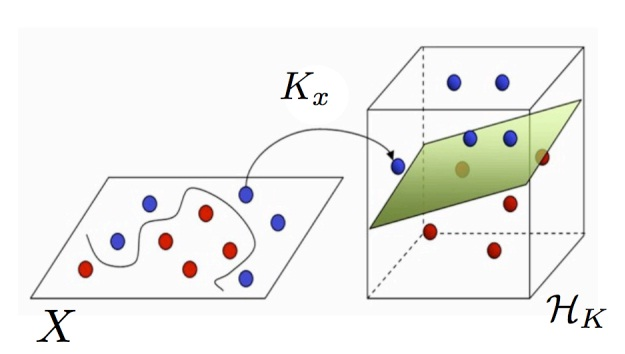
\includegraphics[width=90mm]{featuremaphilbert.jpg}
\caption{Feature map in RKHS}
\label{overflow}
\end{figure}

\section{Ejemplos de RKHS}

\begin{description}
\item[Kernel Lineal:] $K(x,y) = <x,y>$

\item[Kernel Gausiano:] $K(x,y) = e^{-\frac{||x-y||^2}{\sigma^2}}, \sigma > 0$

\item[Kernel polinomial:] $K(x,y) = (<x,y>+1)^d, d \in \mathbb{N}$

\end{description}


\section{Kernel Trick}

\begin{mydef}
Dado un algoritmo formulado en términos de un kernel positivo definido $k$, se puede construir un algoritmo alternativo reemplazando $k$ por otro kernel positivo definido $\tilde{k}$.
\end{mydef}




\newpage
\section{Ejemplo}

Se tiene un espacio de entrada $X=\mathbb{R}^2$ donde sus elementos no son linealmente separables. Se desea llevar los elementos de $X$ a un espacio de características $H=\mathbb{R}^3$ mediante $\Phi$ donde los elementos en $H$ si sean linealmente separables. Entonces se tiene:

\begin{eqnarray*}
\Phi: \mathbb{R}^2=X &\hookrightarrow &H=\mathbb{R}^3 \\
x=(x_1,y_2) &\rightarrow & \Phi(x):=(x_1^2,\sqrt{2}x_1 x_2,x_2^2)
\end{eqnarray*}

También se denomina $\Phi(x)=k_x$.


\begin{figure}[ht!]
\centering
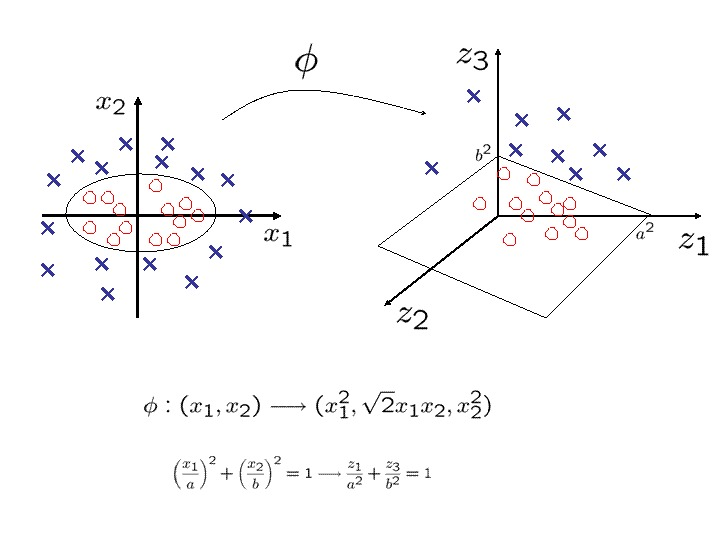
\includegraphics[width=100mm]{ejemplo.jpg}
\caption{Ejemplo de kernel}
\label{ejemplo}
\end{figure}

El espacio de Hilbert $H$ está dado por las funciones $\{f:\mathbb{R}^2 \rightarrow \mathbb{R}\}$ definidas como:

\begin{eqnarray*}
f: \mathbb{R}^2 &\rightarrow& \mathbb{R} \\
x &\rightarrow& f(x) = \langle (a,b,c), \Phi(x)\rangle \\
& & f(x) = a x_1^2 + b x_2 ^2 + c \sqrt{2} x_1 x_2
\end{eqnarray*}

\noindent con $a,b,c \in \mathbb{R}$, donde ahora $f \in H$ puede ser representado por:

\begin{equation}
f= (a,b,c)
\end{equation}

Para este ejemplo la función de kernel se define como:


\begin{eqnarray*}
K: X \times X &\rightarrow &H=\mathbb{R}^3 \\
    (x,y) &\rightarrow & K(x,y):=k_x(y) =\langle k_x, k_y \rangle =\langle \Phi(x), \Phi(y) \rangle = \langle (x_1^2,\sqrt{2}x_1 x_2,x_2^2),(y_1^2,\sqrt{2}y_1 y_2,y_2^2) \rangle \\
    & & =  x_1^2 y_1^2 + 2x_1x_2y_1 y_2 + x_2^2 y_2^2 \\
    & & = (\langle x,y \rangle)^2
\end{eqnarray*}










\newpage
\section{Definiciones}
\label{sec:def}

\begin{mydef}
Sea $X$ un $\mathbb{K}$-espacio vectorial ($\mathbb{K}=\mathbb{C}$ o $\mathbb{R}$). Una \textbf{forma hermitiana} p.d. sobre $X$ es una aplicación:

\begin{eqnarray*}
\langle \cdot, \cdot \rangle: X \times X &\rightarrow & \mathbb{K} \\
  (x,y)&\rightarrow & \langle x,y \rangle
\end{eqnarray*}

Que cumple con las siguientes propiedades:

\begin{enumerate}

\item Es aditiva con respecto al primer argumento:
$$ \langle x + x',y \rangle ) \langle x,y \rangle + \langle x',y \rangle \forall x,x',y \in X$$

\item Propiedad de Homotecia:

$$\langle \alpha x ,y \rangle = \alpha \langle x,y \rangle \forall \alpha \in \mathbb{K} $$

\item Anticonmutatividad

$$ \langle x,y \rangle = \overline{\langle y,x \rangle} \forall x,y \in X$$

\end{enumerate}


Como consecuencia se tiene:

\begin{enumerate}
\item Es aditiva con respecto al segundo argumento
$$\langle x,y + y' \rangle = $$

\item Sesquilineal

\item 
\end{enumerate}

Para $\mathbb{K}=\mathbb{R}$ las formas hermitianas son simplemente formas bilineales simétricas: $\langle x,y \rangle= \langle y,x \rangle$.

Además,

\begin{itemize}
\item $\langle \cdot, \cdot \rangle$ es \textbf{positiva definida}  ssi $\langle x,x \rangle > 0 \forall x \in X$, con $x \neq 0$

\item $\langle \cdot, \cdot \rangle$ es \textbf{positiva semidefinida}  ssi $\langle x,x \rangle \geq 0 \forall x \in X$ (podría existir $u \in X, u\neq 0, \langle u, u \rangle = 0 $)

\item $\langle \cdot, \cdot \rangle$  es \textbf{un producto interno o producto punto} ssi $\langle \cdot, \cdot \rangle$ es \textbf{positiva definida}.
\end{itemize}

\end{mydef}

\textbf{Ejemplo.} Determinar un producto interno, distinto al producto punto canónico.

\emph{Desarrollo.} Sea $X=\mathbb{R}^2$, $A \in Mat(2\times 2, \mathbb{R})$,

\begin{eqnarray*}
\varphi: \mathbb{R}^2  &\rightarrow & \mathbb{R} \\
  (x,y)&\rightarrow & \varphi(x,y) := x^{T}Ay
\end{eqnarray*}

$\varphi$ es positiva definida $\Leftrightarrow \varphi(x,y) > 0 \ \ \forall x, y \in \mathbb{R}^2 \backslash \{0\}$

$\Leftrightarrow x^{T}Ay > 0 \ \ \forall x,y \in \mathbb{R}^2 \backslash \{0\}$

$\Leftrightarrow A$ es positiva definida.

$\Leftrightarrow A=\begin{bmatrix} a & b \\ c & d\end{bmatrix}$


Para que la matriz $A$ es positiva definida (p.d.) si sus subdeterminantes son positivo definidos:  $a>0$ y $ad-bc > 0$

$A=\begin{bmatrix} 1 & 3 \\ 0 & 2 \end{bmatrix}$ es p.d. $\Rightarrow x^{T}Ay = \begin{bmatrix} x_1 & x_2\end{bmatrix}\begin{bmatrix} 1 & 3 \\ 0 & 2 \end{bmatrix} \begin{bmatrix} y_1 \\ y_2 \end{bmatrix} = \begin{bmatrix} x_1 & x_2\end{bmatrix} \begin{bmatrix} y_1 + 3y_2 \\ 2 y_2 \end{bmatrix} = x_1y_1 + 3x_1 y_1 + 2 x_2 y_2$ 


$A=\begin{bmatrix} 1 & 0 \\ 0 & 1 \end{bmatrix}$ es p.d.

$\Rightarrow x^{T}Ay = \begin{bmatrix} x_1 & x_2\end{bmatrix}\begin{bmatrix} 1 & 0 \\ 0 & 1 \end{bmatrix} \begin{bmatrix} y_1 \\ y_2 \end{bmatrix} = x_1 y_1 + x_2 y_2 = \langle x ,  y \rangle_{euclid.}$ 

Por lo tanto,

\begin{eqnarray*}
\varphi: \mathbb{R}^2  &\rightarrow & \mathbb{R} \\
  (x,y)&\rightarrow & \varphi(x,y) := x_1y_1 + 3x_1y_2 +  2x_2y_2 
\end{eqnarray*}

es una forma bilineal p.d. 

$\Rightarrow ||x||_{\varphi}^2 = \varphi(x,y)=x_1 y_1 + 3x_1 y_2 + 2 x_2 y_2$

\begin{mydef}
Un funcional de evaluación sobre el espacio de funciones $H$ es un funcional lineal $L_x: H \rightarrow \mathbb{R}$ que evalúa cada función en $H$ en el punto $x$:

\begin{eqnarray*}
L_x: H &\rightarrow &\mathbb{R} \\
 f &\rightarrow & L_x(f):= f(x)
\end{eqnarray*}
\end{mydef}



\begin{thebibliography}{9}

\bibitem{smola}
  Bernhard Scholkopf and Alexander J. Smola. 
   \emph{Learning with Kernels: Support Vector Machines, Regularization, Optimization, and Beyond.}.
  MIT Press, Cambridge, MA, USA, 
  2001
  
\end{thebibliography}


\end{document}
